\documentclass{article}
\title{CS310 Final Report \\ The Use of Gamification and Analytics in Higher Education}
\author{William Seymour, Third Year Computer Science \\ Supervisor: Mike Joy}
\date{\today}
\linespread{1.3}

\usepackage{cite}
\usepackage{graphicx}
\usepackage{url}

\begin{document}
\maketitle
\clearpage
\tableofcontents

\section{Abstract}
Gamification and analytics are becoming increasingly popular in many facets of everyday life. They are making a big impact in primary and secondary education, driven by the increased use of internet enabled devices in the classroom. This project looks at how this can be translated to higher education, and what role the traditional gamification personality types might have in this field.

\section{Key words}
Gamification, Classroom analytics, Higher education, Flipped classroom

\section{Introduction}
Having becoming an increasingly influential forces in the marketing world over previous years, this report focusses on the educational uses of gamification and analytics. The benefit of integrating these techniques into primary and secondary education was clear from the onset, but there has been less enthusiasm for their use in higher education. This report will assess the usefulness of the aforementioned techniques in the higher education sector, and what form they might take when used to greatest effect. The main body will explore the application of the traditional Bartle personality types used in gamification, with particular interest in how useful (or not) they might be in directing teaching and learning.

Gamifications recent discovery has meant that far less has been done to incorporate developments on it into the current education system than might be possible at some future point. The project starts with a look at how these techniques are being integrated into the current primary and secondary education sectors successfully, and well as analysing some of the opportunities that have been missed. Moving on to Higher education, after examining current work the differences between the two sectors in the context of the applications of gamification and analytics will be investigated. Once it has been established that the fields are sufficiently different that copying over implementations from primary and secondary education will bear little fruit, a rational appraisal of more effective applications will be had. It is important to take a through look at the current state of education before considering the possible impact of game personality types as they provide an important frame of reference for what is quite a specific part of the solution.

\section{Background}
\subsection{What is Gamification?}
It seems an obvious fact of life that work is dull, and play is fun. Many attempts have been made to change this, but they have largely been met with little success. Over the past few years, gamification has been slowly blurring the lines of what is considered to be `work' by moving it towards practises and behaviours that would normally be associated with play. This has all come out of a field of study which is fairly young, the term having only really gained popularity in late 2010, as shown in figure \ref{usagegraph}. Coupled with the advanced user tracking and analytics offered by modern technology, it has begun to dominate the way in which we interact electronically, with services like Facebook and Foursquare being prime examples.

At its core, it is the idea of taking the elements which have made traditional games provided fun and entertainment for all of human history, and using them to transform everyday tasks which many find less interesting. While the results so far of gamified experiences are very promising, with many use cases reporting exponential increases in customer attraction and retention \cite{zichermann2010game}, there are some ethical questions raised due to the fact that gamification often takes the form of operant conditioning \cite{kapp2012gamification}. While manipulating users in order to stimulate learning is often lauded as being virtuous, using it to sell products and make a profit is not. This will be explored more in section \ref{sec:issues}.

\subsection{How does it work?}
The success of gamification in driving engagement has underlying roots in psychology, with gameified experiences being able to satisfy more psychological needs than what might normally be considered `work'. For example, the feedback mechanisms which typify these experiences, such as progress bars, badges and the awarding of in-game points, help fulfil the need for competence experienced by all human beings \cite{przybylski2010motivational}. Players are compelled to complete game actions in order to feel capable, and challenges often use time investment as the principal measure of worth. Traditional games tend to confer rewards and status based on skill, which alienates a large proportion of the player base who fall outside the top performers. In this way all players feel as if they can succeed if they play the game for long enough, or regularly enough.

As mentioned above, a key part of the psychology behind gamification is that of operant conditioning. Introduced as a concept by B.F. Skinner, it focuses on conditioning organisms to perform tasks that they would not normally undertake. In his experiments, Skinner would place pigeons in boxes and reward them with food whenever they pushed a button in their cage. If every push pf the button resulted in a reward, the birds would stop pecking as soon as the food stopped being dispensed. He found that when rewards were awarded on a semi random basis, the animals would continue to peck at the buttons long after the food was gone \cite{kapp2012gamification}. This form of conditioning is used to great effect in many forms of gambling, and is the reason gamblers will continue to insert coins into machines in the hope that they might get that elusive win. Indeed, it seems counterintuitive that reducing the frequency of rewards might actually increase uptake by users. It turns out that chasing a win or payoff with slim odds is for more exciting than completing an action with a known reward. In fact, it may well be that the act of achieving a rare reward is motivation in itself, even if there is no real world value attached to it.

\subsection{High profile usage of gamification}
As gamification expands more and more into everyday life, each sector is asking the question of how they can keep up. To a certain extent, a change of thinking is required. Increasingly is is becoming a question of why should people be expected to stop having fun in order to learn, watch an advertisement or communicate? \cite{zichermann2010game} Or, put more bluntly, why would they? The rise of gamification has meant that other forms of experience are less effective than they once were, just by virtue of the new competition. What follows are a pair of case studies of gamification employed by high profile organisations to serve as a practical example of what exactly gamification and analytics mean in the context of the modern day, and proof of how effective they can be when used to their full potential.

\subsubsection{Case Study: Orkut}

An early example of the power of gamification can be seen in Orkut, the social networking site which was developed by Google in early 2004. Orkut was different from other social networks available at the time in that users had profiles operating on three different levels. Information provided by users was divided up into personal, professional and social, but more interestingly, Orkut would provide a list of demographics about the current user population \cite{fragoso2006wtf}. It was one such demographic that began a completely unexpected phenomenon in Brazil. In an attempt to climb to the top of the perceived leaderboard, blogs and posts started appearing all over Brazillian internet sites \cite{zichermann2010game}.  By June 2004 the number of Brazillian users had surpassed those from the United States to take the top spot on the usage demographics. What had begun as an interesting statistic had motivated thousands of people to become invested in a product to such an extent that Orkuts domination of the Brazilian social network scene did not end until December 2012 \cite{1_comscore_2012}.

\begin{figure}
	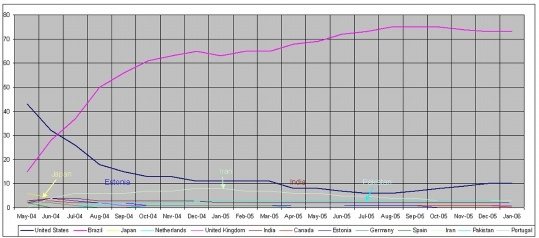
\includegraphics{../img/orkut-brazil.jpg}
	\caption{Orkut usage by country, shown for the top ten coutries among Orkuts user population. Data from May 2004 to January 2006 \cite{fragoso2006wtf}.}
	\label{orkut-brazil}
\end{figure}

\subsubsection{Case Study: ABC}

\begin{figure}
	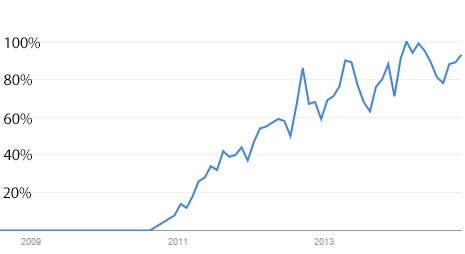
\includegraphics{../img/usage-graph.png}
	\caption{Usage of the term `gamification' by month as a proportion of the total number of Google searches for gamification, from 2009 to the present day \cite{usage}.}
	\label{usagegraph}
\end{figure}

\section{Definitions}
It is important to define some of the key terms that will be used in this report. Terms like gamification and analytics are often bandied around by lots of different parties who all mean similar but subtly different things. Indeed, the way in which these terms have been used thus far have been somewhat unclear. For the remainder of the document, the undermentioned should be referred to as a definitive explanation of what is meant by the following technical terms:

\subsection{Gamification}
A commonly accepted definition of gamification is that it is the use of game design elements in non-game contexts \cite{deterding2011game}. This is a good in that it makes clear the distinction between games and gamified activities, but what exactly counts as either can often be left unclear. This is difficult as it is near impossible to pin down where one stops and the other begins. This is likely to increase as game elements are further incorporated into everyday activities, and seems to suggest that rigorously defining what is and is not a game is of less value than originally anticipated. Here, a game [man, play and games put on hold].

Game elements also need to be outlined in a little more depth. For the purposes of this project, it will be taken to mean those elements of game systems which compel users to play because they are engaging or fun. Alternatively put, the focus is on the mechanics that make games interesting and keep users coming back as opposed to graphical techniques or the platforms they reside on. This  Further definition, as before, carries the risk of splitting hairs, and does not add much to the discussion.

\subsection{Analytics}
The other component to the project is analytics, with a focus on online learning platforms. In this context analytics refers to feedback systems which collect data on various facets of the learning process. Crucially, they must provide information which can then be used to improve the process further and better understand the dynamics of class makeup and teaching styles, under analysis by either the system itself or a human analyst. This is to provide some differentiation between software which merely reports back statistics such as student or class scores, with no extra dimension by which the effectiveness of the setup as a whole can be bettered. 

Tracking and comparing different sets of statistics in this way shows correlations that might otherwise be missed. Singling out these links is the key to effective improvement of higher education. It is not required for the purposes of this definition that the analysis be automated and carried out by the system itself. In many small scale implementations, such as the one used for this project, the resources available preclude the development of sych an advanced piece of software. Indeed, implementing a prototype smart learning platform would be financially expensive for many institutions, and excluding them would have a negative impact on the data that could be obtained.

In the research carried out for this report, the correlation between Bartle's gamer personality types and individual learning styles was assessed, with the view of recommending how they might fit in to a more optimal model of gamified higher education. As such, the software developed for the project uses preliminary content with pre-defined Bartle weighting to gauge a users gamer type. As required in the paragraph above, this can be combined with other heuristics in order to answer the questions set forth by the project. 

\section{Primary and Secondary Education}

\section{How is Higher Education Different?}

\section{Higher Education}

\section{Bartle Personality Types}

\section{Methodology}

\section{Findings}

\section{Evaluation}

\section{Conclusion and Further Work}

\section{Legal, Social, Ethical and Professional Issues}
\label{sec:issues}

\section{Background Texts}

\bibliography{references}
\bibliographystyle{plain}
\end{document}